% 2005 年江西卷理科第 7 题题干图：y = x f'(x) 图象
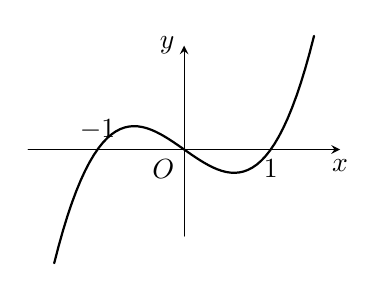
\begin{tikzpicture}[>=stealth,scale=1.1,line cap=round]
  \draw[->] (-1.8,0) -- (1.8,0) node[below] {$x$};
  \draw[->] (0,-1.0) -- (0,1.2) node[left] {$y$};
  \node[below left] at (0,0) {$O$};
  \draw[thick,domain=-1.5:1.5,samples=60] plot (\x,{\x*(\x*\x - 1)*0.7});
  \node[above] at (-1,0) {$-1$};
  \node[below] at (1,0) {$1$};
\end{tikzpicture}
